% -----------------------------------------------------------------------------
% Modelo de apresentação de trabalho acadêmico
% Projeto hospedado em: https://github.com/cfgnunes/latex-slides
%
% Autor: Cristiano Fraga G. Nunes <cfgnunes@gmail.com>
% -----------------------------------------------------------------------------

\documentclass[aspectratio=34, 12pt]{latex-slides}
%\documentclass[aspectratio=34, 12pt, faixa_superior]{latex-slides}

\usepackage[%
    alf,
    abnt-emphasize=bf,
    bibjustif,
    recuo=0cm,
    abnt-doi=expand,       % Expande endereço DOI para http://dx.doi.org/
    abnt-url-package=url,  % Utiliza o pacote url
    abnt-refinfo=yes,      % Utiliza o estilo bibliográfico abnt-refinfo
    abnt-etal-cite=3,
    abnt-etal-list=3,
    abnt-thesis-year=final
]{abntex2cite}             % Configura as citações bibliográficas

% -----------------------------------------------------------------------------
% Pacotes utilizados
% -----------------------------------------------------------------------------
\usepackage[utf8]{inputenc}     % Codificação do documento
\usepackage[T1]{fontenc}        % Seleção de código de fonte
\usepackage[brazil]{babel}      % Configuração de idioma
\usepackage[algoruled, portuguese]{algorithm2e}  % Algoritmos em português
\usepackage{amssymb, amsmath}   % Fontes e símbolos matemáticos
\usepackage{graphicx}           % Inclusão de gráficos
\usepackage{multirow, array}    % Tabelas com múltiplas linhas e colunas
\usepackage{verbatim}           % Exibir texto tal como escrito no documento
\usepackage[scaled]{helvet}     % Usa a fonte Helvetica
\usepackage{caption}            % Caption de objetos
\usepackage{leading}            % Espaçamento entre linhas
\usepackage{ragged2e}           % Justificação do documento

% -----------------------------------------------------------------------------
% Configurações gerais
% -----------------------------------------------------------------------------

% Configura o label das figuras
\captionsetup[figure]{labelformat=simple}

% Para justificação global
\renewcommand{\raggedright}{\leftskip=0pt \rightskip=0pt plus 0cm}

% Redefine a fonte para uma fonte similar a Arial (fonte Helvetica)
\renewcommand*\familydefault{\sfdefault}

% Preâmbulo
\title{Título do trabalho}
\author{Cristiano Fraga Guimarães Nunes}
\institute[CEFET-MG]{%
    \par\vspace{1em}
    Centro Federal de Educação Tecnológica de Minas Gerais
    \par\vspace{1em}
}
\date{01 de janeiro de 2020}

% -----------------------------------------------------------------------------
% Início do documento
% -----------------------------------------------------------------------------
\begin{document}

% Configura o espaçamento entre linhas
\leading{1.5em}

% -----------------------------------------------------------------------------
% Capa
% -----------------------------------------------------------------------------

\begin{frame}
    \titlepage
\end{frame}

% -----------------------------------------------------------------------------
% Sumário
% -----------------------------------------------------------------------------

\begin{frame}
    \frametitle{Sumário}

    \tableofcontents
\end{frame}

% -----------------------------------------------------------------------------
% Introdução
% -----------------------------------------------------------------------------

\section{Introdução}

\begin{frame}
    \frametitle{Introdução}

    \begin{itemize}
        \item Inserir seu texto aqui...
        \item Inserir seu texto aqui...
    \end{itemize}
\end{frame}

% -----------------------------------------------------------------------------
% Caracterização do problema
% -----------------------------------------------------------------------------

\begin{frame}
    \frametitle{Caracterização do problema}

    \setcounter{figure}{3}
    \begin{figure}[!t]
        \centering
        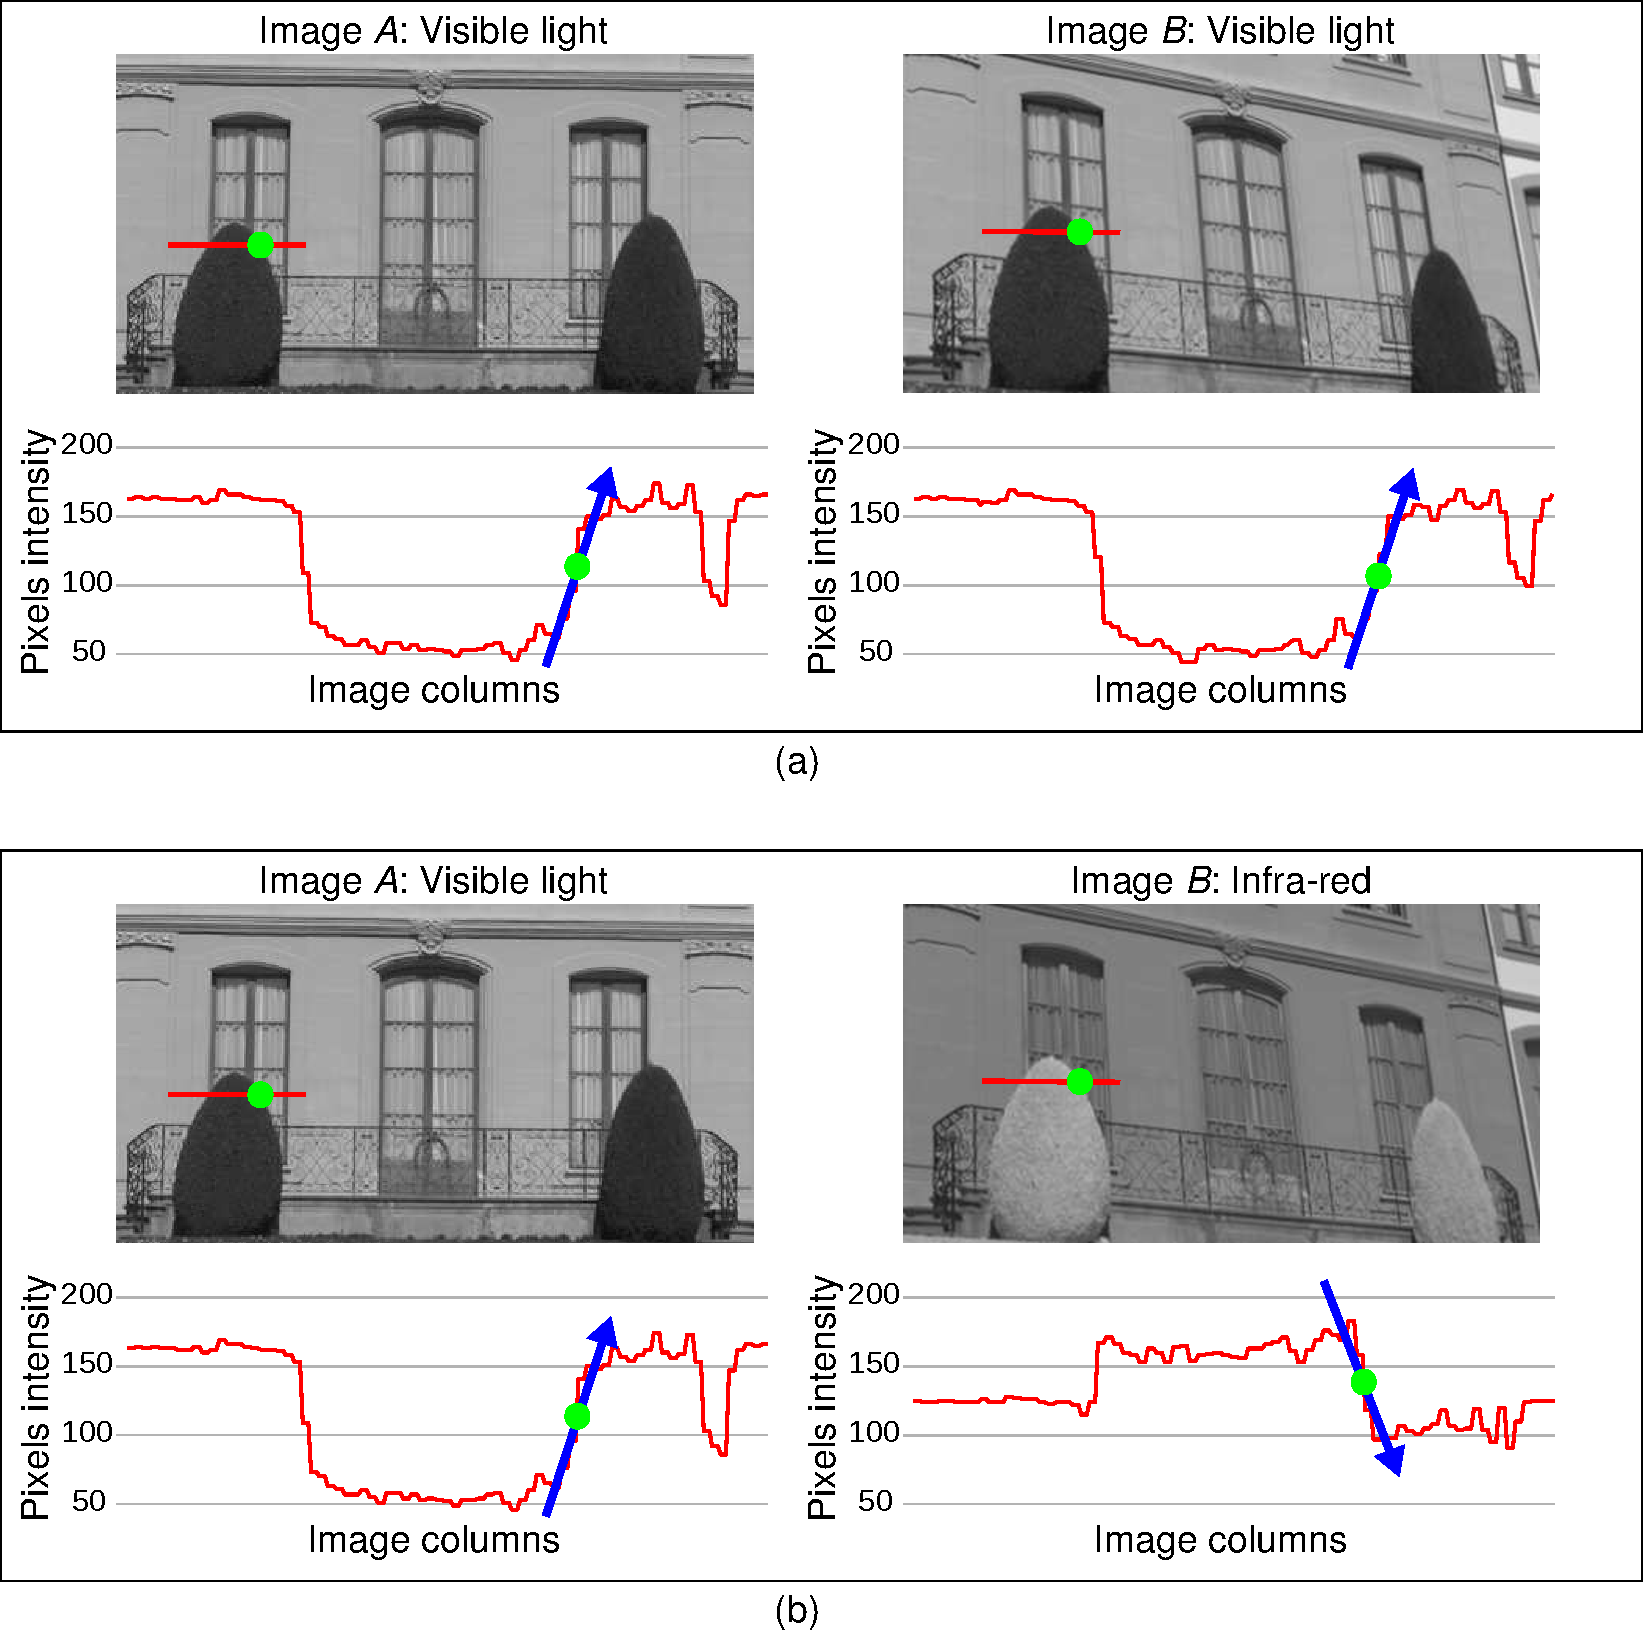
\includegraphics[width=0.55\textwidth]{./figuras/figura-exemplo1}
        \caption{Exemplo de figura.}
        \label{fig:exemplo_figura}
    \end{figure}
\end{frame}

\begin{frame}
    \frametitle{Caracterização do problema}

    \begin{itemize}
        \item Inserir seu texto aqui... \cite{nunes2017local}
        \item Inserir seu texto aqui...
    \end{itemize}
\end{frame}

% -----------------------------------------------------------------------------
% Motivação
% -----------------------------------------------------------------------------

\begin{frame}
    \frametitle{Motivação}

    \begin{itemize}
        \item Inserir seu texto aqui...
        \item Inserir seu texto aqui...
    \end{itemize}

\end{frame}

% -----------------------------------------------------------------------------
% Trabalhos Relacionados
% -----------------------------------------------------------------------------

\section{Trabalhos Relacionados}

\begin{frame}
    \frametitle{Trabalhos Relacionados}

    \begin{itemize}
        \item Inserir seu texto aqui...
        \item Inserir seu texto aqui...
    \end{itemize}
\end{frame}

% -----------------------------------------------------------------------------
% Fundamentação Teórica
% -----------------------------------------------------------------------------

\section{Fundamentação Teórica}

\begin{frame}
    \frametitle{Fundamentação Teórica}

    \begin{itemize}
        \item Inserir seu texto aqui...
        \item Inserir seu texto aqui...
    \end{itemize}
\end{frame}

\begin{frame}
    \frametitle{Métricas de avaliação}

    \begin{itemize}
        \item Inserir seu texto aqui...
        \item Inserir seu texto aqui...
    \end{itemize}
\end{frame}

% -----------------------------------------------------------------------------
% Metodologia
% -----------------------------------------------------------------------------

\section{Metodologia}

\begin{frame}
    \frametitle{Metodologia}

    \begin{itemize}
        \item Inserir seu texto aqui...
        \item Inserir seu texto aqui...
    \end{itemize}
\end{frame}

% -----------------------------------------------------------------------------
% Resultados
% -----------------------------------------------------------------------------

\section{Resultados}

\begin{frame}
    \frametitle{Base de dados para avaliação}

    \begin{itemize}
        \item Inserir seu texto aqui...
        \item Inserir seu texto aqui...
    \end{itemize}
\end{frame}

% -----------------------------------------------------------------------------
% Conclusão
% -----------------------------------------------------------------------------

\section{Conclusão}

\begin{frame}
    \frametitle{Conclusão}

    \setcounter{figure}{3}
    \begin{figure}[!t]
        \centering
        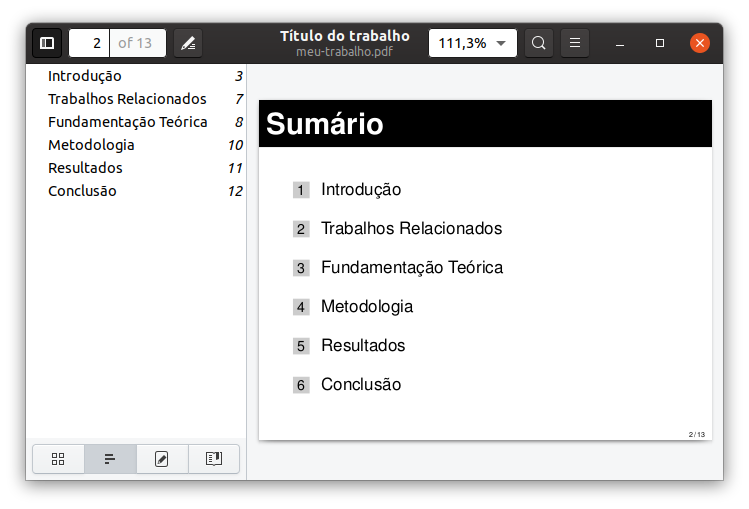
\includegraphics[width=0.55\textwidth]{./figuras/figura-exemplo2}
        \caption{Outro exemplo de figura.}
        \label{fig:outro_exemplo_figura}
    \end{figure}
\end{frame}

% -----------------------------------------------------------------------------
% Referências
% -----------------------------------------------------------------------------

\begin{frame}[allowframebreaks]
%\begin{frame}<presentation:0>[noframenumbering]
    \frametitle{Referências}

    \scriptsize
    \bibliography{referencias.bib}
\end{frame}

% -----------------------------------------------------------------------------
% Capa
% -----------------------------------------------------------------------------

\begin{frame}
    \titlepage
\end{frame}

\end{document}
